\subsection{\lya\ forest lensing}


For the first probe, the \lya\ forest,  the \atf\ will be measured
from the large-scale structure of the intergalactic medium, as 
seen in quasar spectra.  
The forest has the advantage of spectral information,
potentially yielding many lensed ``slices'' at different redshifts.
An idealized test was carried out in C18 using using a mock high
resolution angular grid of quasars (of order arcminute separ\ ation)
and a linear theory foreground density field. Standard quadratic
estimators (e.g., \cite{okamoto}) were used to successfully
reconstruct images of the foreground mass distribution. In the work
proposed here we will expand the realism of such tests and make
measurements on real data. Enough work has been done to  date on this
source that this is a relatively low risk project. There is still the
question of how powerful a tool \atf\ of the \lya\ \ forest statistics
will become. Will they surpass the more traditional shape
measurements for at least some range of redshift? What are the
systematics that must be treated in order to extract cosmological
information? We argue below that we are well-suited to address these
questions and feel that they provide a broad range of opportunities
for graduate students.


\subsubsection{The \lya\ forest as a tracer of structure}

The \lya\ forest of absorption features due to neutral hydrogen can
seen in the spectra of both quasars \cite{rauch1998} and galaxies (e.g.,
\cite{savaglio2002}).  We refer to quasars and galaxies as
``backlights'' rather than ``sources'' in what follows, in order to
avoid confusion with the ``sources'' in gravitational lensing (which
will be the \lya\ forest here). At the redshifts ($2 < z
< 6$) where the \lya\ transition is in the optical wavelength
range, the forest absorption mostly arises in the moderately overdense
(of order the cosmic mean) intergalactic medium (IGM) (\cite{bi1993}, 
\cite{cen1994}, \cite{zhang1995}, \cite{hernquist1996}).
  This intergalactic medium is a continuous field, and as such
\lya\ forest spectra can be thought of as a collection of
one-dimensional ``intensity maps'',
where the relevant property is the ``flux overdensity'', $\df=\frac{F}{\langle F \rangle} -1$ ($F$
is the transmitted flux in a spectrum).  Its properties are well
studied and it is relatively easy to simulate numerically (see e.g.,
\cite{bolton2017}). The forest has been used to test
cosmological models, for example through the influence of the neutrino
mass on large-scale structure (e.g., \cite{pal2015}, \cite{croft1999}).
  With a high enough angular
density of quasars, three dimensional statistics can be evaluated by
using information from multiple sightlines, enabling clustering
measurements and detection of baryon
oscillations \citep{busca2013},. The
collection of one-dimensional skewers can also be used to make
continuous three dimensional maps using a variety of interpolation
techniques (e.g., \cite{cisewski}), and
with even more numerous star forming galaxies as background spectra
these can be made with angular resolution close to arcminute scales
\citep{Lee2014}.

The \lya\ forest, being measured from spectra has a precisely known
source redshift. This fact is also advantageous for lensing of the
CMB, enabling analyses to be free of uncertainties in the redshift
distribution of sources which affect galaxy weak lensing studies
\citep{hearin2010}.

\subsubsection{Lenses for the forest}

The \lya\ forest at redshift $z_{s}$ is lensed by the matter
distribution lying between us and $z_{s}$. Gravitational lensing
shifts the observed positions of points on the sky without changing
their surface brightness.  In the case of the \lya\ forest, this means
that the quasar or galaxy backlights move on the plane of the sky.
The angular sizes of quasars are magnified (through the change in
their angular sizes). This magnification of quasars through lensing is
well studied, from the first observed lenses, which created multiple
quasar images \citep{walsh1979}, through weak lensing
magnification of quasars detected by cross-correlation with foreground
galaxies (e.g., \cite{scranton2005}).  The magnification of
quasars will cause some selection biases which we plan to investigate
with mocks. Directly relevant to \lya\ forest lensing, however
are distortions of the angular separations between quasars, caused by
the lensing deflection of light. 
  Gravitational lensing therefore distorts the ``image'' of the 
IGM probed by the \lya\ forest without
changing the transmitted flux measured in each pixel. This is directly
analogous to the effect of lensing on 21cm emission (or the CMB),
which conserves surface brightness.  In
the left panel of Figure \ref{cartoon} we
illustrate this with a diagram, which shows the \lya\ forest pixels
being deflected in a similar fashion to the quasar backlights. In
the right panel of 
Figure \ref{cartoon} we concentrate on a single backlight and \lya\
forest pixel and show the relationship to the unlensed angular
positions of both. The pixel and the backlight are at different
angular size distances, and so are displaced on the sky by different
angles.

\begin{figure}
  \begin{center}
    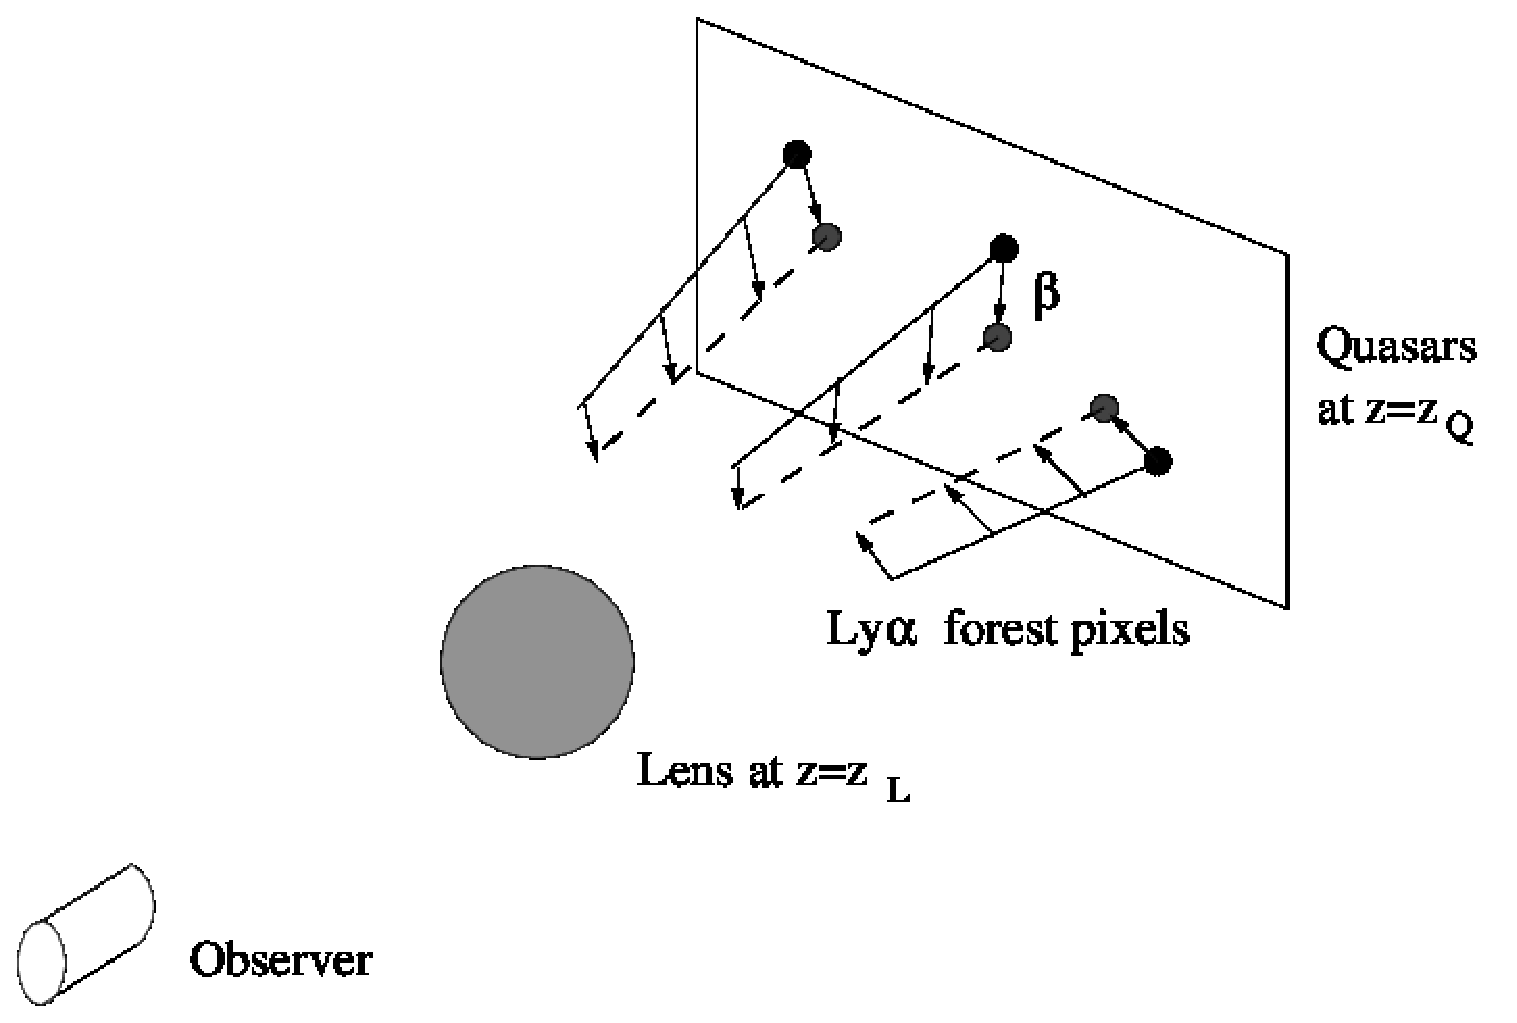
\includegraphics[scale=0.33]{figs/lensdiagram.eps}
    \hspace{1cm}
    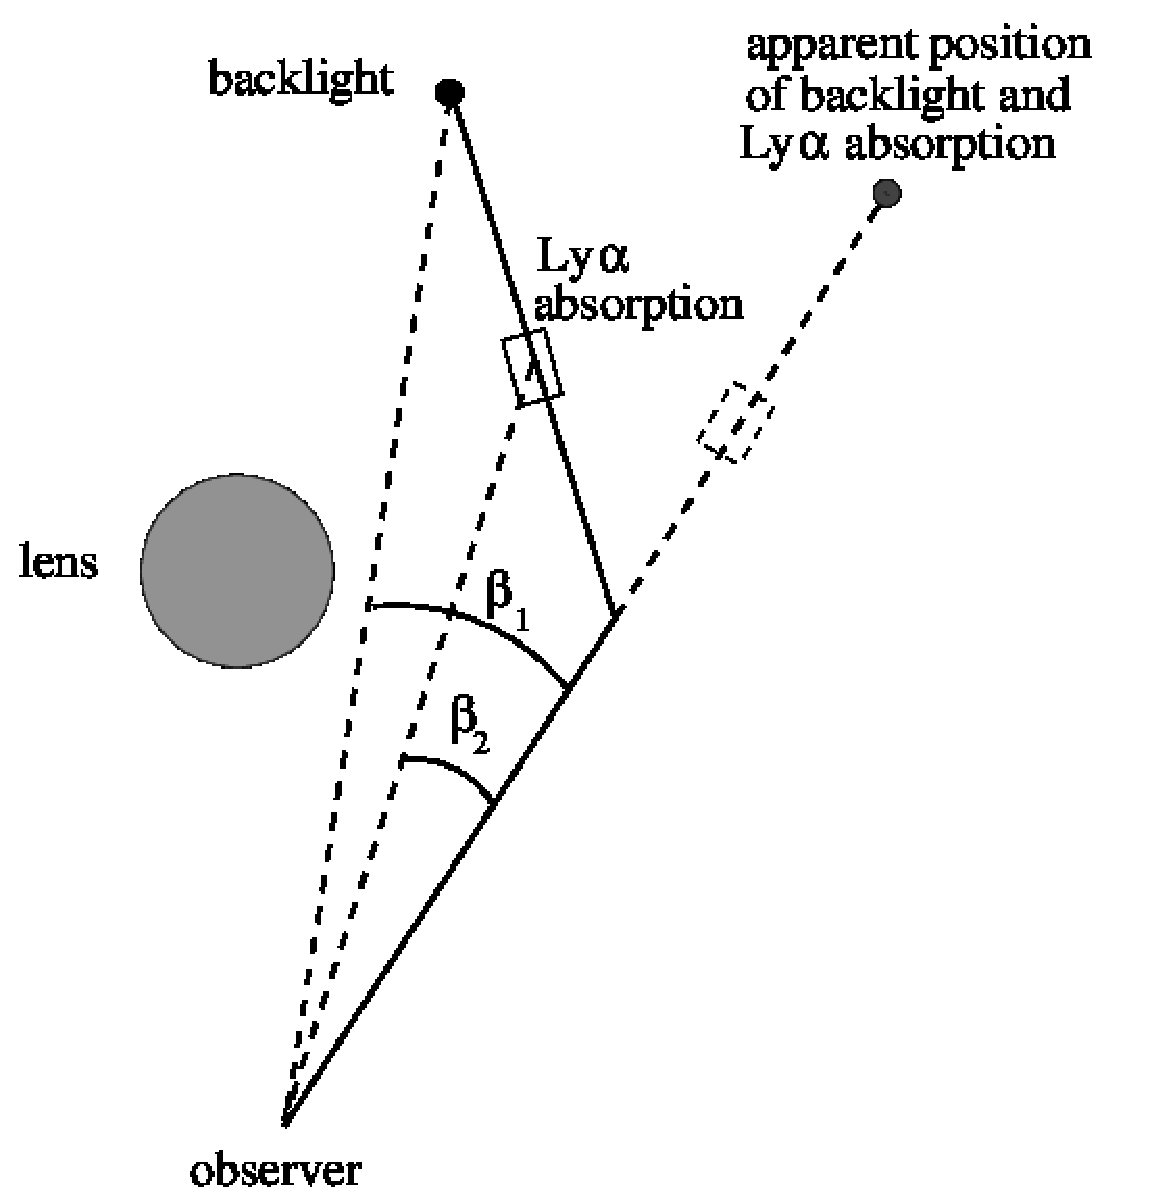
\includegraphics[scale=0.33]{figs/angdiag.eps}
  \end{center}
  \caption{ \footnotesize
{\bf Left panel: cartoon illustration of the geometry of \lya\ forest lensing.}
Due to lensing by the foreground object at redshift $z_{L}$, the 
angular position of a quasar at redshift $z=z_{Q}$ is 
deflected by an angle $\beta$. The associated
\lya\ forest pixels are also lensed, deflected by an angle smaller than 
$\beta$ 
(which depends on the angular size distance to the absorption in the pixel).
{\bf Right panel: lensing deflection for a single \lya\ forest pixel.}
The deflection angle for the backlight ($\beta_{1}$) is different 
from that for the \lya\ forest absorption    ($\beta_{2}$) because they are 
at different redshifts (and                       therefore angular size distances).
           }
  \label{cartoon}
\end{figure}


If the lensing deflections are small
compared to structure in the source, the \lya\ forest 
flux overdensity $\df$  at wavelength $\lambda$ can
be expressed as a Taylor expansion of the unlensed $\df$.

\begin{equation}
\widetilde{\delta}_{F}({ \pmb {\theta}},\lambda)=
{\delta_{F}}({ \pmb {\theta}} - {\pmb { \alpha}}({\pmb {\theta}}) ,\lambda)
\simeq {\delta_{F}} ({\pmb{\theta}},\lambda) - {\pmb {\alpha}}({\pmb{\theta}})\c
dot
{\pmb{\nabla_{\theta}}} \delta_{F} ({\pmb{\theta}},\lambda) + ...
%\delta_{F}({\bf \theta-\alpha(\theta)}, \lambda) 
%\simeq \delta_{F}({\bf \theta},\lambda)
\label{taylor}
\end{equation}

 This expansion is  valid in the case of the \lya\ forest, where gradients
in $\delta_{F}$ can be large, but the deflections (or deflection gradients) 
are small compared to them on all scales of interest. The deflection field
${\pmb {\beta}}( {\pmb {\theta}})$ is related to the 2D projected lensing potent
ial via
${\pmb {\nabla \Phi}} =- {\pmb {\beta}}({\pmb {\theta}} )$,
in the weak lensing limit. This lensing potential can be
computed from the full 3D gravitational
potential (e.g, Bartelmann \& Schneider 2001) by an integration
over redshift as in \ec{phi}.
This lensing potential
can  be reconstructed from the \lya\ forest field using 
quadratic estimators (e.g., \cite{okamoto}).

